%% PNAStmpl.tex
%% Template file to use for PNAS articles prepared in LaTeX
%% Version: Apr 14, 2008


%%%%%%%%%%%%%%%%%%%%%%%%%%%%%%
%% BASIC CLASS FILE 
%% PNAStwo for two column articles is called by default.
%% Uncomment PNASone for single column articles. One column class
%% and style files are available upon request from pnas@nas.edu.
%% (uncomment means get rid of the '%' in front of the command)

%\documentclass{pnasone}
\documentclass{pnastwo}
\bibliographystyle{pnas}
%%%%%%%%%%%%%%%%%%%%%%%%%%%%%%
%% Changing position of text on physical page:
%% Since not all printers position
%% the printed page in the same place on the physical page,
%% you can change the position yourself here, if you need to:

% \advance\voffset -.5in % Minus dimension will raise the printed page on the 
                         %  physical page; positive dimension will lower it.

%% You may set the dimension to the size that you need.

%%%%%%%%%%%%%%%%%%%%%%%%%%%%%%
%% OPTIONAL GRAPHICS STYLE FILE

%% Requires graphics style file (graphicx.sty), used for inserting
%% .eps files into LaTeX articles.
%% Note that inclusion of .eps files is for your reference only;
%% when submitting to PNAS please submit figures separately.

%% Type into the square brackets the name of the driver program 
%% that you are using. If you don't know, try dvips, which is the
%% most common PC driver, or textures for the Mac. These are the options:

% [dvips], [xdvi], [dvipdf], [dvipdfm], [dvipdfmx], [pdftex], [dvipsone],
% [dviwindo], [emtex], [dviwin], [pctexps], [pctexwin], [pctexhp], [pctex32],
% [truetex], [tcidvi], [vtex], [oztex], [textures], [xetex]

\usepackage{graphicx}

%%%%%%%%%%%%%%%%%%%%%%%%%%%%%%
%% OPTIONAL POSTSCRIPT FONT FILES

%% PostScript font files: You may need to edit the PNASoneF.sty
%% or PNAStwoF.sty file to make the font names match those on your system. 
%% Alternatively, you can leave the font style file commands commented out
%% and typeset your article using the default Computer Modern 
%% fonts (recommended). If accepted, your article will be typeset
%% at PNAS using PostScript fonts.


% Choose PNASoneF for one column; PNAStwoF for two column:
%\usepackage{PNASoneF}
%\usepackage{PNAStwoF}

%%%%%%%%%%%%%%%%%%%%%%%%%%%%%%
%% ADDITIONAL OPTIONAL STYLE FILES

%% The AMS math files are commonly used to gain access to useful features
%% like extended math fonts and math commands.

\usepackage{amssymb,amsfonts,amsmath}

%%%%%%%%%%%%%%%%%%%%%%%%%%%%%%
%% OPTIONAL MACRO FILES
%% Insert self-defined macros here.
%% \newcommand definitions are recommended; \def definitions are supported

%\newcommand{\mfrac}[2]{\frac{\displaystyle #1}{\displaystyle #2}}
%\def\s{\sigma}


%%%%%%%%%%%%%%%%%%%%%%%%%%%%%%
%% Don't type in anything in the following section:
%%%%%%%%%%%%
%% For PNAS Only:
\contributor{Submitted to Proceedings
of the National Academy of Sciences of the United States of America}
\url{www.pnas.org/cgi/doi/10.1073/pnas.0709640104}
\copyrightyear{2008}
\issuedate{Issue Date}
\volume{Volume}
\issuenumber{Issue Number}
%%%%%%%%%%%%

\begin{document}

%%%%%%%%%%%%%%%%%%%%%%%%%%%%%%


%% For titles, only capitalize the first letter
%% \title{Almost sharp fronts for the surface quasi-geostrophic equation}

\title{Efficient inference using the approximate Riemannian geometry of stochastic population models}


%% Enter authors via the \author command.  
%% Use \affil to define affiliations.
%% (Leave no spaces between author name and \affil command)

%% Note that the \thanks{} command has been disabled in favor of
%% a generic, reserved space for PNAS publication footnotes.

%% \author{<author name>
%% \affil{<number>}{<Institution>}} One number for each institution.
%% The same number should be used for authors that
%% are affiliated with the same institution, after the first time
%% only the number is needed, ie, \affil{number}{text}, \affil{number}{}
%% Then, before last author ...
%% \and
%% \author{<author name>
%% \affil{<number>}{}}

%% For example, assuming Garcia and Sonnery are both affiliated with
%% Universidad de Murcia:
%% \author{Roberta Graff\affil{1}{University of Cambridge, Cambridge,
%% United Kingdom},
%% Javier de Ruiz Garcia\affil{2}{Universidad de Murcia, Bioquimica y Biologia
%% Molecular, Murcia, Spain}, \and Franklin Sonnery\affil{2}{}}

\author{Ben Calderhead\affil{1}{University College London, London, United Kingdom}, Colin S. Gillespie\affil{2}{Newcastle University, Newcastle upon Tyne, United Kingom}}
% \email{b.calderhead@ucl.ac.uk}
% \email{colin.gillespie@newcastle.ac.uk}
% \\
% 	   Centre for Mathematics and Physics in the Life Sciences and Experimental Biology,\\University College London, UK
% 	   \and 
% 	   School of Mathematics \& Statistics, Newcastle University,
% 	   NE1 7RU, UK
\contributor{Submitted to Proceedings of the National Academy of Sciences
of the United States of America}

%% The \maketitle command is necessary to build the title page.
\maketitle

%%%%%%%%%%%%%%%%%%%%%%%%%%%%%%%%%%%%%%%%%%%%%%%%%%%%%%%%%%%%%%%%
\begin{article}

\begin{abstract} -- enter abstract text here -- \end{abstract}


%% When adding keywords, separate each term with a straight line: |
\keywords{moment closure | stochastic | inference}

%% Optional for entering abbreviations, separate the abbreviation from
%% its definition with a comma, separate each pair with a semicolon:
%% for example:
%% \abbreviations{SAM, self-assembled monolayer; OTS,
%% octadecyltrichlorosilane}

% \abbreviations{}

%% The first letter of the article should be drop cap: \dropcap{}
%\dropcap{I}n this article we study the evolution of ''almost-sharp'' fronts

%% Enter the text of your article beginning here and ending before
%% \begin{acknowledgements}
%% Section head commands for your reference:
%% \section{}
%% \subsection{}
%% \subsubsection{}

\section{Useful Papers}

\begin{itemize}
\item Papers cited in \textbf{refs.bib}
\item Useful papers put in papers directory
\end{itemize}



\section{Introduction}
\label{s:intro}\textbf{31/8: BC/CSG}

\begin{itemize}
\item Inference for MJP is difficult: non-linear likelihood, computational
  expensive, proposals expensive, analytically intractable likelihood
\item Data: Partially observed discrete, noisy time-course.
\item Existing work for likelihood evaluations: 
\begin{itemize}
\item Likelihood calculations
\begin{itemize}
\item Exact: Boys et al, slow, not noise
\item Approx SDE - Andy and Darren (with Noise)
\item Approx MC - Andy and Colin (no noise)
\item Approx LNA - Mark (no noise), Kolmo' (no noise, but check)
\end{itemize}
\end{itemize}
\item Novel stuff
\end{itemize}
Different from Mark's LNA paper:
\begin{itemize}
\item Analysis of impact of the approximate proposal scheme
\item Using Noise
\item Using delayed acceptance scheme so exact inference
\item Time course data
\item Using real data
\end{itemize}

Importance of stochastic population models for further scientific understanding of natural systems vs deterministic models.  For example in ecology, where we often have to deal with discrete noisy data.  Importance of parametric sensitivity has already been shown for determining vital properties of biological systems such as robustness and also in experimental design where the sensitivity gives information about the identifiability of individual rate constants.

The sensitivity of parameters is also of central importance when inferring unknown parameter values for a mathematical model

Performing exact inference over stochastic kinetic models described by Markov Jump Processes is extremely difficult.  First and foremost, the likelihood is usually analytically intractable for models with levels of complexity suitable for describing natural phenomena.

Approximations of the likelihood surface, such as LNA and moment closure.  Parameter inference - want to explore the likelihood surface - can consider it as a Riemannian manifold.  This manifold is an approximation of the true underlying Riemannian manifold of the analytically intractable likelihood.

non-linear likelihood, computational expensive, proposals expensive, analytically intractable likelihood



\section{Methods}

\subsection{Stochastic Population Models}

C \& B

\subsection{Moment Closure Scheme}

CSG

\subsection{Approximate Riemannian Geometry}
BC

\subsection{Delay Acceptance Scheme}

?
Key point: little overhead for approximate likelihood


\section{Example}

\subsection{Immigration-death}

  \begin{itemize}
  \item Calculate exact proposal for comparison (\textbf{17/8: CSG})
  \item Construct LNA model for ID (\textbf{14/9: CSG/BC})
  \item Graphs:
    \begin{itemize}
    \item Data: \textbf{17/8: CSG}
    \item Geometry proposal: 3 proposals for the 3 derviates: k1\^2, k1k2, k2\^2
      \textbf{24/8: }
    \item Likelihood: Exact likelihood vs LNA vs MC \textbf{24/8: }
    \item Delay acceptance(?)
    \item Sampling efficiences M-H vs RM (appendix)
    \end{itemize}
  \end{itemize} 
  
\subsection{SIR (type) model}


    \begin{itemize}
    \item Construct moment equations (\textbf{17/8: CSG}) Lognormal?
    \item Construct proposal
    \item Delay acceptance
    \item Run experiments
    \item Graphs:
      \begin{itemize}
      \item Data
      \item Sampling efficiences M-H vs RM (appendix)
      \item Posterior compare to Stumpf
      \end{itemize}
    \end{itemize}

\subsection{Aphid data set}

\subsubsection{Introduction}

36 parameters - 18 birth, 18 death. 3 water treatments, 3 nitrogen treatments
and 3 blocks, with interactions. 5*27 (I think) latent data sets. Exploit Sub-mannifolds for choosing parameter sets
Poisson error structure. 


    \begin{itemize}
    \item Construct moment equations (appendix) \textbf{Done}
    \item Construct proposal (appendix)
    \item Delay acceptance
    \item Run experiments
    \item Graphs:
      \begin{itemize}
      \item Data \textbf{Done}
      \item Sampling efficiences M-H vs RM; ESS
      \item Posteriors
      \end{itemize}
    \end{itemize}
    
\section{Discussion}

\begin{itemize}
\item Use of geometry vital in tackling real problems
\item Could also use other approximation schemes such as the LNA??
\end{itemize}

%% == end of paper:

%% Optional Materials and Methods Section
%% The Materials and Methods section header will be added automatically.

%% Enter any subheads and the Materials and Methods text below.
%\begin{materials}
% Materials text
%\end{materials}


%% Optional Appendix or Appendices
%% \appendix Appendix text...
%% or, for appendix with title, use square brackets:

%Taken from the tex file in the docs folder
%Not edited yet
\appendix[Immigration-death process]


This model has a single species, $N(t)$. The first reaction represents a constant immigration rate, and occurs with rate $k_1$. The second reaction represents death in the $N$ population and occurs with rate $k_2 N(t)$. The model can be represented by the coupled (pseudo) reactions, 
\begin{equation}\label{1}
R_1: \emptyset  \xrightarrow{\phantom{a}k_1\phantom{a}} N 
\quad \text{and} \quad
R_2: N  \xrightarrow{\phantom{a}k_2\phantom{a}} \emptyset.
\end{equation}
The forward Kolmogorov equation (or CME) for this model is
\[
dp_{n}(t)/dt = k_1 p_{n-1}(t) +  k_2 (n+1) p_{n+1}(t) 
- (k_1 + k_2 n) p_{n}(t) \;.
\]
This equation can be solved exactly using a generating function approach.

\subsection{Moments}

The general idea of \textit{moment closure} is to represent the analytically intractable moments of the process as a set of ODEs. The solutions of these ODEs provide approximations for the moments. With this particular system, we can solve the ODEs analytically - so the moments are exact.

The marginal means of the process are:
\[
E[n(t) | n(0) = n_0 ] = \frac{k_1}{k_2}(1-e^{-k_2 t}) + n_0 e^{-k_2 t} \;.
\]
Notice that as $t \rightarrow \infty$,
\[
E[n(t) | n(0) = n_0 ] = \frac{k_1}{k_2} \;.
\]
The marginal variance is
\[
Var[n(t) | n_0]  = \left(\frac{k_1}{k_2} + n_0e^{-k_2 t}\right)(1-e^{-k_2 t}) \;.
\]


%Just copied from the RSS paper
\appendix[Aphid model]


Following \cite{Matis06}, we assume a linear aphid population birth rate of $\lambda N(t)$ where $N(t)$ denotes the size of the aphid population at time $t$. As discussed in \cite{Prajneshu98}, aphids excrete honey-dew, forming a cover on the leaf surface and causing aphid starvation. As the area covered by excretion at time $t$ is proportional to the cumulative population size at time $t$, $C(t)$, we assume a death rate of $\mu N(t)C(t)$ and for simplicity, assume that there is no removal or decomposition of honey-dew \cite{Matis06,Matis07a,Matis08}. The model can be represented by the coupled (pseudo) reactions, 
\begin{align}
N & \xrightarrow{\phantom{a}\lambda\phantom{a}} 2N + C \label{2.1} \\
N+C & \xrightarrow{\phantom{a}\mu\phantom{a}} C \label{2.2}
\end{align}
since clearly, an occurrence of (\ref{2.1}) will lead to a unit increase in both $N$ and $C$ whereas the reaction in  (\ref{2.2}) will give a unit decrease in $N$ but leave $C$ unchanged. Such models are known in the literature as stochastic kinetic models; see \cite{Wilkinson06} for a concise introduction. We can express the probabilistic laws governing the time evolution of the process by considering a small interval $(t,t+dt]$, namely
\begin{align}
\Pr\left\{N(t+dt)=n(t)+1,\,C(t+dt)=c(t)+1\,|\,n(t),c(t)\right\}&=\lambda n(t)dt+o(dt) \label{2.3} \\
\Pr\left\{N(t+dt)=n(t)-1,\,C(t+dt)=c(t)\,|\,n(t),c(t)\right\}&=\mu n(t)c(t)dt+o(dt),\label{2.4}
\end{align}
and we adopt the convention that upper case denotes random variable and lower case denotes the realisation. The expressions in (\ref{2.3}) and (\ref{2.4}) describe a Markov jump process where each event occurs at a particular rate dependent on the current state of the system. Note that ignoring stochasticity leads to a deterministic model where the time course behaviour of $N(t)$ and $C(t)$ is described by the set of differential equations,
\[
\left\{\begin{array}{l}
\displaystyle\frac{dN(t)}{dt}=\lambda N(t)-\mu N(t)C(t)\\
\\
\displaystyle\frac{dC(t)}{dt}= \lambda N(t)
\end{array}\right.
\] 



\begin{acknowledgments}
Thanks to AG and Ohio state University
\end{acknowledgments}

%% PNAS does not support submission of supporting .tex files such as BibTeX.
%% Instead all references must be included in the article .tex document. 
%% If you currently use BibTeX, your bibliography is formed because the 
%% command \verb+\bibliography{}+ brings the <filename>.bbl file into your
%% .tex document. To conform to PNAS requirements, copy the reference listings
%% from your .bbl file and add them to the article .tex file, using the
%% bibliography environment described above.  

%%  Contact pnas@nas.edu if you need assistance with your
%%  bibliography.

% Sample bibliography item in PNAS format:

\bibliography{refs}    
%% Enter the largest bibliography number in the facing curly brackets
%% following \begin{thebibliography}

%  \begin{thebibliography}{}
% % \bibitem{in-text reference} comma-separated author names up to 5,
% % for more than 5 authors use first author last name et al. (year published)
% % article title  {\it Journal Name} volume #: start page-end page.
% % ie,
% \bibitem{Neuhaus} Neuhaus J-M, Sitcher L, Meins F, Jr, Boller T (1991) 
% A short C-terminal sequence is necessary and sufficient for the
% targeting of chitinases to the plant vacuole. 
% {\it Proc Natl Acad Sci USA} 88:10362-10366.
%  
%  \end{thebibliography}

\end{article}
%%%%%%%%%%%%%%%%%%%%%%%%%%%%%%%%%%%%%%%%%%%%%%%%%%%%%%%%%%%%%%%%

%% Adding Figure and Table References
%% Be sure to add figures and tables after \end{article}
%% and before \end{document}

%% For figures, put the caption below the illustration.
%%
%% \begin{figure}
%% \caption{Almost Sharp Front}\label{afoto}
%% \end{figure}

%% For Tables, put caption above table
%%
%% Table caption should start with a capital letter, continue with lower case
%% and not have a period at the end
%% Using @{\vrule height ?? depth ?? width0pt} in the tabular preamble will
%% keep that much space between every line in the table.

%% \begin{table}
%% \caption{Repeat length of longer allele by age of onset class}
%% \begin{tabular}{@{\vrule height 10.5pt depth4pt  width0pt}lrcccc}
%% table text
%% \end{tabular}
%% \end{table}

%% For two column figures and tables, use the following:

%% \begin{figure*}
%% \caption{Almost Sharp Front}\label{afoto}
%% \end{figure*}

%% \begin{table*}
%% \caption{Repeat length of longer allele by age of onset class}
%% \begin{tabular}{ccc}
%% table text
%% \end{tabular}
%% \end{table*}

\begin{figure}[ht]
\begin{center}
\centerline{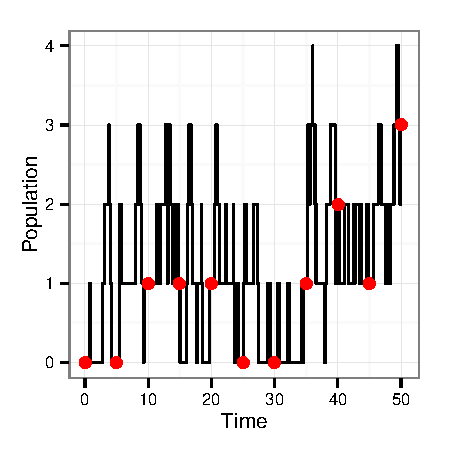
\includegraphics[]{../graphics/figure1}}
\end{center}
\caption{Stochastic simulation of the immigration-death process, with parameters
$k_1=k_2=1$ and $n(0)=0$. The black line shows the full stochastic realisation, 
the red dots indiciate the observed data.}\label{F1}
\end{figure}
\begin{figure*}[ht]
\begin{center}
\centerline{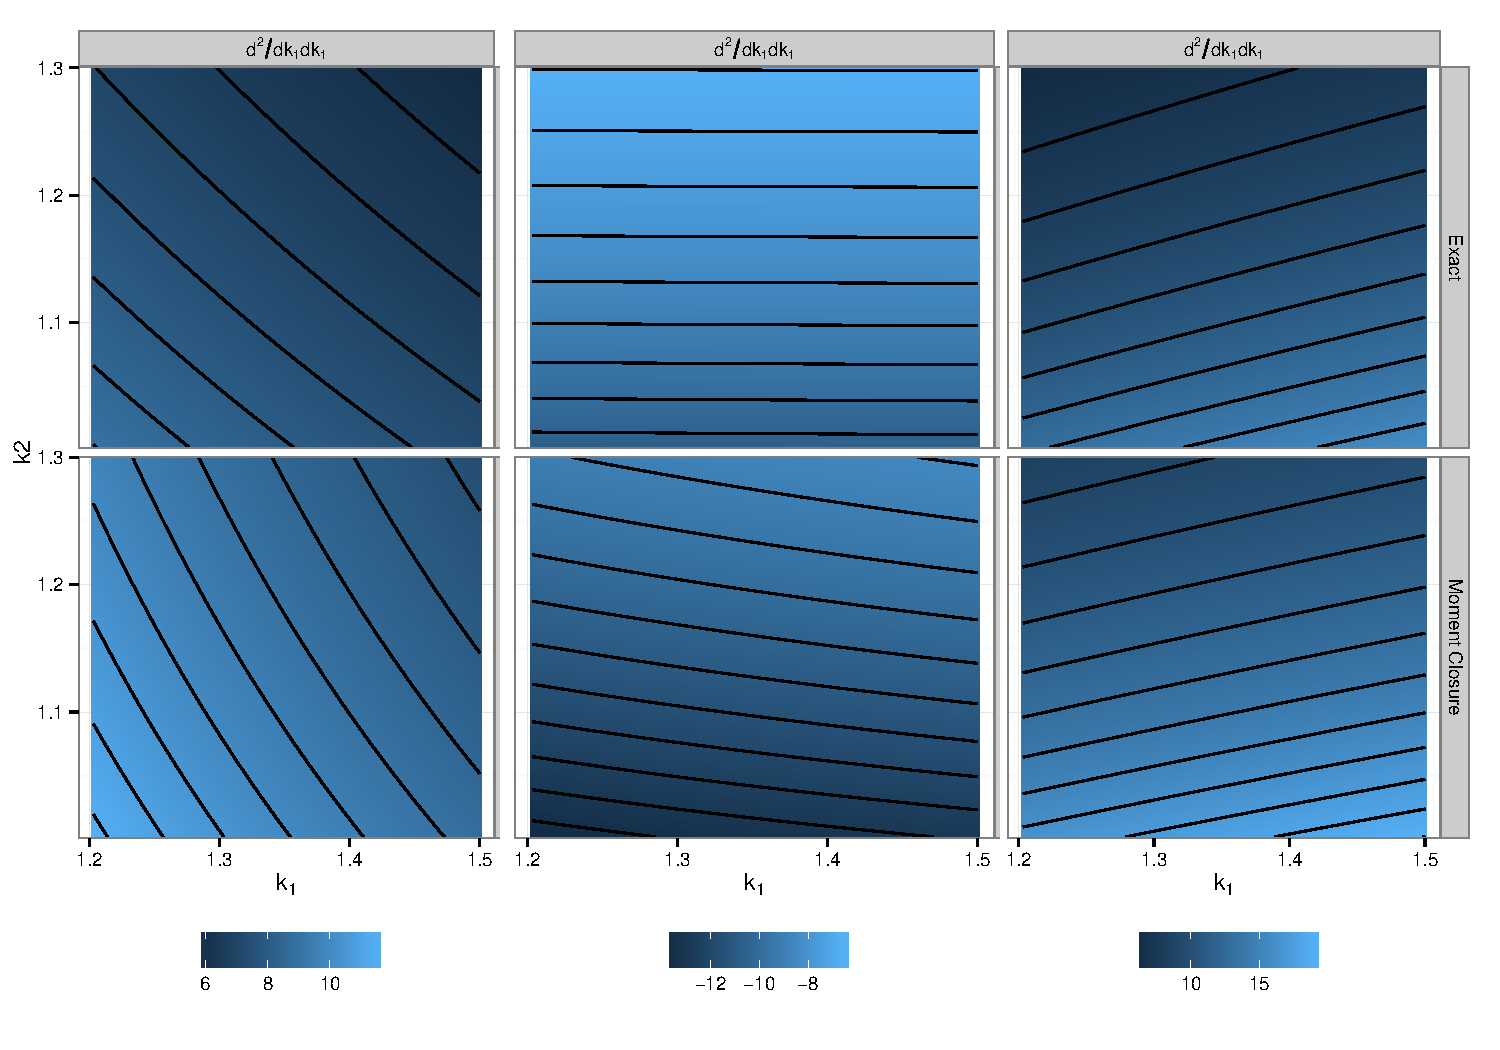
\includegraphics[width=.7\textwidth]{../graphics/figure2}}
\caption{Comparison of the exact and the moment closure expected fisher information matrix. }
\label{F2}
\end{center}
\end{figure*}
% 
% \begin{figure*}
% \centering
% 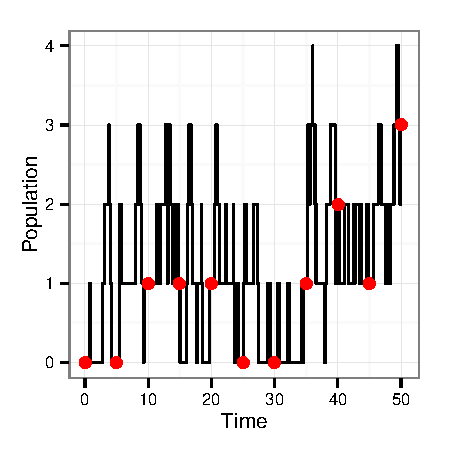
\includegraphics[]{../graphics/figure1}
% \caption{blah}
% \end{figure*}

\end{document}

